%! TEX root = ../thesis.tex
\begin{figure}
	\newcommand{\imgscale}{0.5}
	{%
		\setlength{\fboxsep}{5.5pt}%
		\setlength{\fboxrule}{0.5pt}%
		\fbox{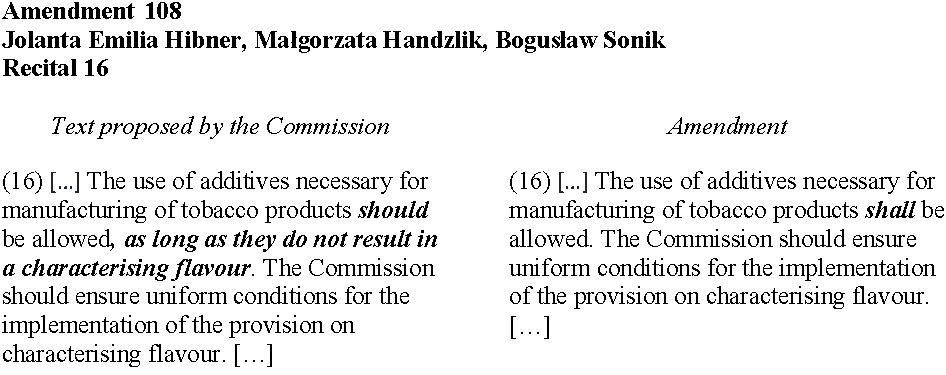
\includegraphics[scale=\imgscale]{lmp-amendment-108}}%
	}%
	\vfill
	\vspace{4pt}
	{%
		\setlength{\fboxsep}{5.5pt}%
		\setlength{\fboxrule}{0.5pt}%
		\fbox{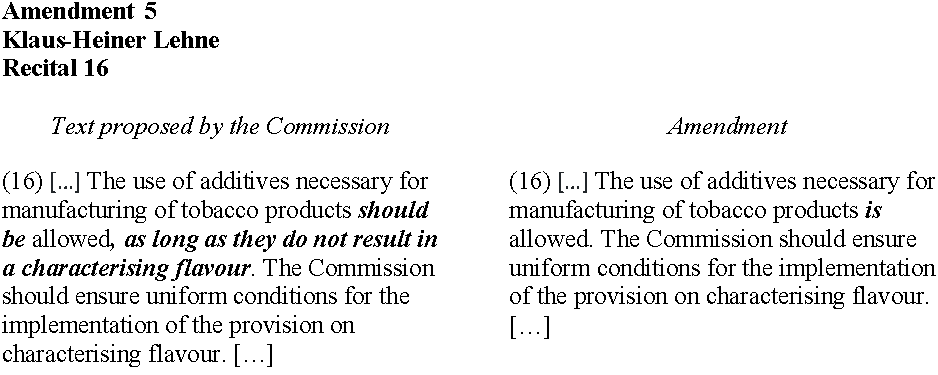
\includegraphics[scale=\imgscale]{lmp-amendment-5}}%
	}%
	\caption{
		Example of two conflicting amendments in their raw format.
		(Top) Am. 108 is proposed by three MEPs on a text legislating tobacco-related products.
		(Bottom) Am. 5 is proposed by another MEP on the same text.
		The two edits of Am. 108, replacing "should" by "shall" and removing the end of the first sentence, are rejected.
		The first edit is in conflict with the first edit of Am. 5, proposing to replace "should be" by "is".
		This edit is also rejected.
	}
	\label{fig:amendment}
\end{figure}

\section{Data}
\label{sec:data}

% Amendments.
We collected a dataset of \numprint{237177} legislative amendments from the European Parliament website.\footnote{Data and code publicly available on \href{https://github.com/indy-lab/war-of-words}{https://github.com/indy-lab/war-of-words}.}
The dataset spans the 7\th legislature~(referred to as EP7), from 2009 to 2014, and the 8\th legislature~(EP8), from 2014 to 2019.
MEPs come from 28 different countries, and they belong to one of the 8 (EP7) or 9 (EP8) political groups.
We show in Figure~\ref{fig:amendment} an example of a raw amendment.
An amendment consists of (i) one or several authors, (ii) the original text by the European Commission, and (iii) the amended text by the author(s).
MEPs propose amendments on a specific article of the legislation, and they can modify several parts within a single amendment.
As a result, we decompose the difference between the original and the amended text into one or several \textit{edits}, as defined below.
We summarize our dataset in Table~\ref{tab:dataset} and we refer to it as the \warofwords\ dataset.
In the next paragraphs, we describe the data that we extract from amendments and that we use for the subsequent analysis.
% We extract \textit{edits} and \textit{conflicts}, and we explain the labelization process.
Technical details about data processing are given in Appendix~\ref{sec:dataproc}.

\begin{figure*}
	\newcommand{\imgscale}{0.88}
	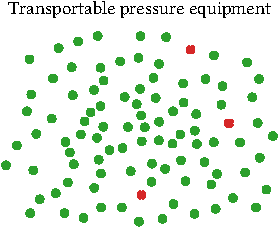
\includegraphics[scale=\imgscale]{lmp-edit-graph-tpe}\hfill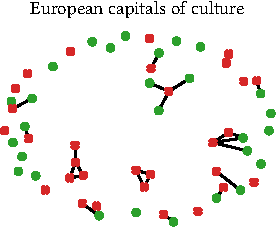
\includegraphics[scale=\imgscale]{lmp-edit-graph-ecc}\hfill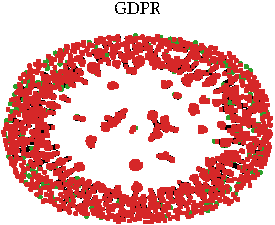
\includegraphics[scale=\imgscale]{lmp-edit-graph-gdpr}
	\caption{
		(Left) The "transportable pressure equipment" edit graph contains 96 edits (97\% accepted) and no conflicts.
		(Center) The "European capitals of culture" edit graph contains 58 edits (48\% accepted) and 16 conflicts.
		(Right) The GDPR edit graph contains 3154 edits (9\% accepted) and 1298 conflicts.
	}
	\label{fig:edit_graph}
\end{figure*}

\paragraph{Edits.}
An edit is a sequence of words that are inserted or deleted or both.
We extract edits by computing the \textit{diff}, i.e., the difference between the words in two texts, between the original and the amended text of each amendment.
We normalize the texts by removing special characters and by putting the words in lower case.
We keep punctuation because the structure of sentences is important in legal texts.
We merge identical edits proposed by different MEPs, thus considering them as one edit proposed by all authors together.
This is in line with the Rules of Procedure of the Parliament \cite{europarl2018rules}.
We extract \numprint{200407} edits for EP7 and \numprint{249086} edits for EP8.
On average, there are 1.85 and 1.93 edits per amendment for EP7 and EP8, respectively.
There are also more dossiers in EP7 than in EP8, which means that there are proportionally more edits per dossier in EP8.

\paragraph{Conflicts}
There exists an inherent competition between the MEPs in the amending process, as amendments are vehicles of political ideas and interests.
We are therefore interested in the conflicts between edits.
We define a \textit{conflict} as a set of edits that overlap.
Edits overlap because they modify parts of the text at the same position.
We extract \numprint{40302} conflicts for EP7 and \numprint{56298} for EP8.
Adding the conflicts to isolated edits, we obtain a dataset of \numprint{126417} data points for EP7 and \numprint{141034} data points for EP8.

\paragraph{Labels}
The votes on each edit are not publicly available, and we need to infer their outcomes from the raw data.
Reports and opinions contain only the amendments accepted within the committees.
Draft reports, draft opinions, and other documents containing all proposed amendments are published separately.
Therefore, if the edits extracted from the latter documents  appear in the former documents, we label them as \textit{accepted}, i.e., the committee votes to include these edits in their report or opinion.
Otherwise, we label them as \textit{rejected}.
Out of the proposed edits, 37.7\% are accepted for EP7 and 25.7\% for EP8.

\paragraph{Timestamps}
The timeline of the legislative process described in Section~\ref{sec:background} varies from one dossier to another.
Depending on the dossier, MEPs can propose edits during a window of one to six months, after which all the edits related to that dossier are published together.
As a result, the actual, detailed chronology of the edits is unfortunately hidden.
Furthermore, there is a delay between the time an edit is proposed and the time it is voted: recent edits might be voted \textit{before} older ones.
The timestamps associated with each edit are, therefore, noisy.

\paragraph{Example of Amendment}
We show in Figure~\ref{fig:amendment} an example of two conflicting amendments in their raw format.
Amendment 108 is proposed on Recital 16 of a legislation on tobacco-related products.
Its authors are three Polish MEPs: Jolanta Emilia Hibner, Małgorzata Handzlik, and Bogusław Sonik.
It consists of two edits:
The first one deletes "should" and inserts "shall"; the second one deletes the end of the first sentence.
Amendment 5 is authored by a German MEP: Klaus-Heiner Lehne.
It consists of two edits:
The first one replaces "should be" by "is"; the second one is identical to the second edit of Amendment 108.
Consequently, the first edits of Amendment 5 and 108 are in conflict, whereas the second edits are identical and are therefore merged, as they are proposed by the four MEPs together.
All these edits were rejected in this case.
This example illustrates nonetheless the subtlety of legislative texts: The difference between "should", "shall", and "is" is crucial \cite{guardian2015typo}.

